\documentclass{beamer}
\usepackage{relsize}
\usepackage{color}

\usepackage{listings}
\usetheme{CambridgeUS}
%\usepackage{beamerthemesplit} % new
\usepackage{enumitem}
\usepackage{amsmath}                    % See geometry.pdf to learn the layout options.
\usepackage{amsthm}                   % See geometry.pdf to learn the layout options. There
\usepackage{amssymb}                    % See geometry.pdf to learn the layout options.
\usepackage[utf8]{inputenc}
\usepackage{graphicx}
\usepackage[english,bulgarian]{babel}

\usepackage{caption}
\usepackage{tikz}

\usetheme{CambridgeUS}
\usecolortheme{crane}

\lstset{language=C++,
                basicstyle=\ttfamily\small,
                keywordstyle=\color{blue}\ttfamily,
                stringstyle=\color{red}\ttfamily,
                commentstyle=\color{green}\ttfamily,
                morecomment=[l][\color{magenta}]{\#}
}

\newtheorem{mydef}{Дефиниция}[section]
\newtheorem{lem}{Лема}[section]
\newtheorem{thm}{Твърдение}[section]

\DeclareMathOperator{\restrict}{\upharpoonright}

\setitemize{label=\usebeamerfont*{itemize item}%
  \usebeamercolor[fg]{itemize item}
  \usebeamertemplate{itemize item}}

\setbeamercovered{transparent}

\captionsetup{font=tiny} 

\begin{document}
\title[Монади]{Монади. Практически поглед}
\frame{\titlepage}

\section{Монади}
\subsection{Maybe}


\begin{frame}[fragile]
  \frametitle{Състояние}

\begin{lstlisting}[language=Haskell]
type Pos = (Int, Int)
  
data Tile = Road | Wall | Gold
            deriving (Show, Eq)
  
data Game = Game { pos :: Pos, world :: [[Tile]]}
            deriving (Show)
  
myWorld :: Game = Game { pos = (0, 0), 
                         world = [[Road, Wall, Gold], 
                                  [Road, Wall, Road], 
                                  [Road, Road, Road]]}
\end{lstlisting}

\begin{tikzpicture}[remember picture,overlay]
  \node[xshift=75mm,yshift=-12mm,anchor=north west] at (current page.north west){%
  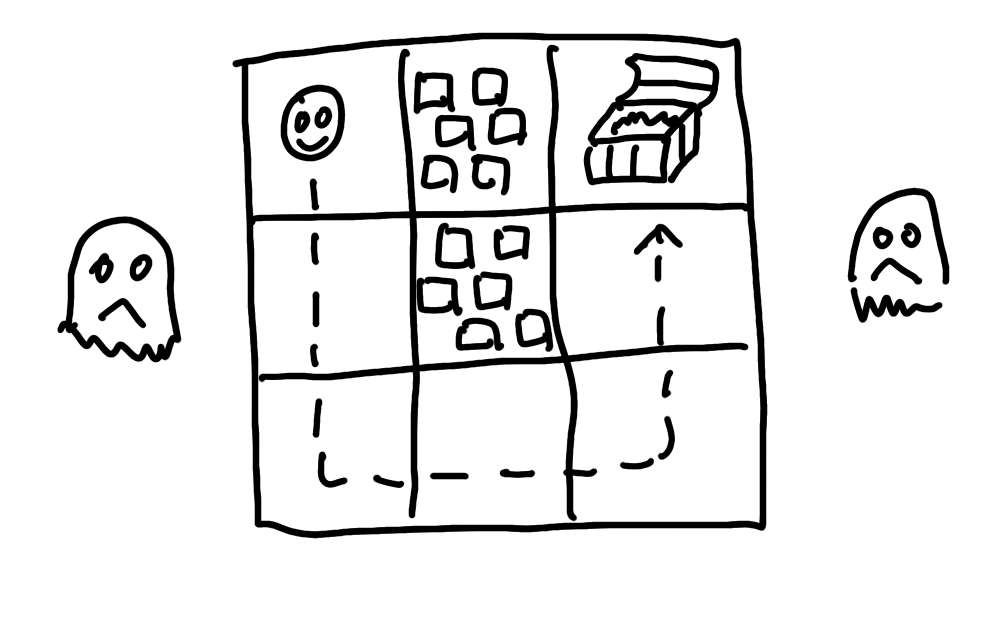
\includegraphics[width=50mm]{images/maze.png}};
\end{tikzpicture}

\end{frame}


\begin{frame}[fragile]
  \frametitle{Операции}

\begin{lstlisting}[language=Haskell]
left (Game (x, y) w) = Game (x-1, y) w
right (Game (x, y) w) = Game (x+1, y) w
up (Game (x, y) w) = Game (x, y-1) w
down (Game (x, y) w) = Game (x, y+1) w
\end{lstlisting}

\end{frame}


\begin{frame}[fragile]
  \frametitle{Композиране на операции}

\begin{lstlisting}[language=Haskell]
walk1 g = (up . up . right . right . down . down) g
\end{lstlisting}

\begin{tikzpicture}[remember picture,overlay]
  \node[xshift=75mm,yshift=-12mm,anchor=north west] at (current page.north west){%
  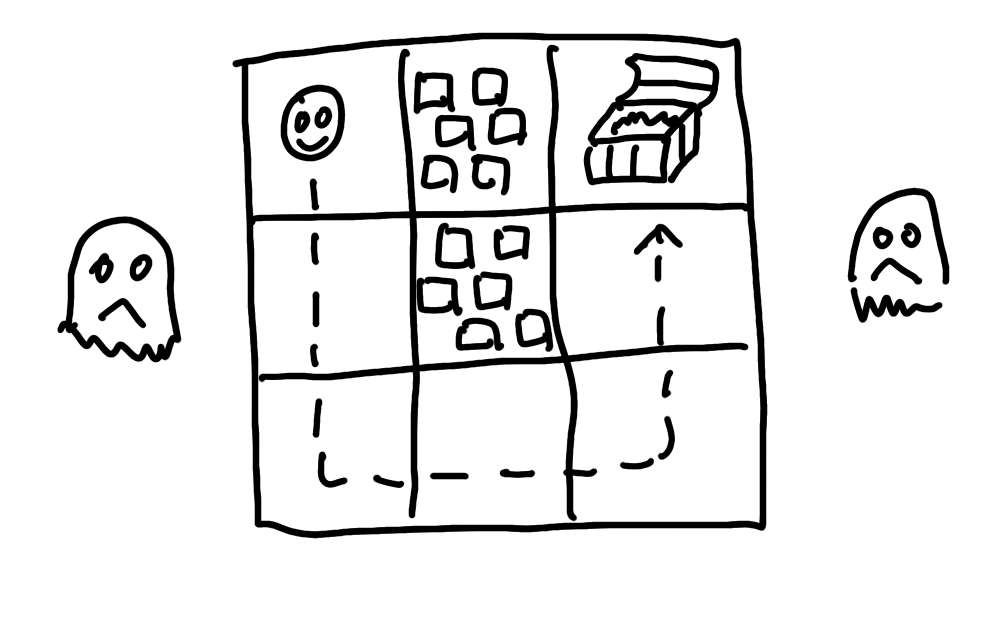
\includegraphics[width=50mm]{images/maze.png}};
\end{tikzpicture}


\end{frame}


\begin{frame}[fragile]
  \frametitle{Композиране на операции}

\bigskip
\bigskip
\bigskip
\bigskip
\bigskip

\begin{lstlisting}[language=Haskell]
walk1 = up . up . right . right . down . down

(->>) :: Game -> (Game->Game) -> Game
g ->> f = f g

walk1 g = g->>down->>down->>right->>right->>up->>up
\end{lstlisting}

\begin{tikzpicture}[remember picture,overlay]
  \node[xshift=75mm,yshift=-12mm,anchor=north west] at (current page.north west){%
  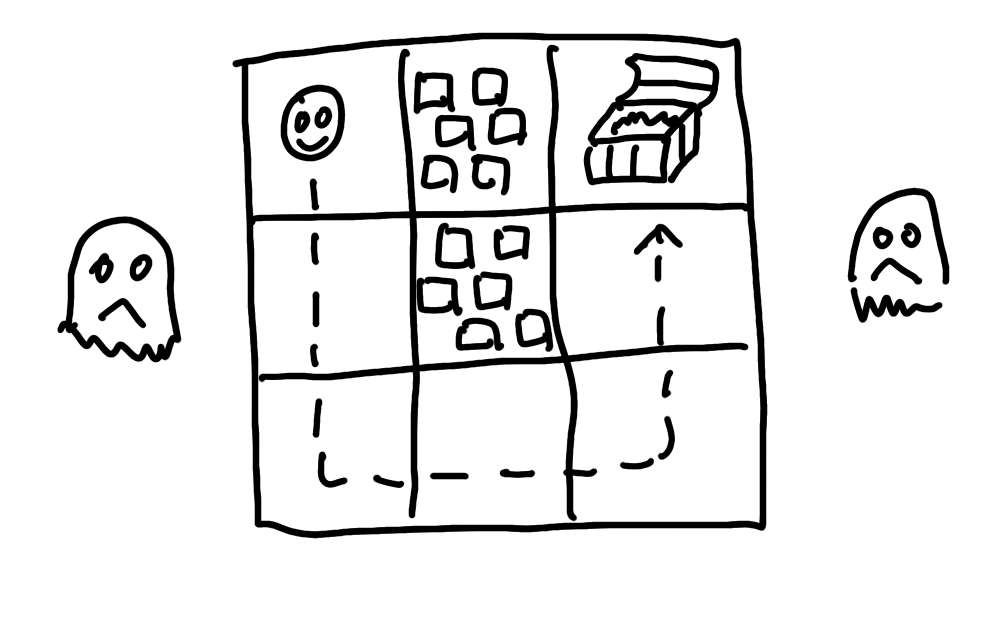
\includegraphics[width=50mm]{images/maze.png}};
\end{tikzpicture}

\end{frame}


\begin{frame}[fragile]
  \frametitle{Грешки}

\begin{lstlisting}[language=Haskell]
dead :: [[Tile]] -> Pos -> Bool
dead w (x, y) = x < 0 || x >= length w ||
                y < 0 || y >= length w || 
                (w !! y) !! x == Wall

left (Game (x, y) w) 
    | dead w (x-1,y) = error "Error, dead player!"
    | otherwise = Game (x-1, y) w

ghci> left myWorld 
*** Exception: Error, dead player!
\end{lstlisting}


\begin{tikzpicture}[remember picture,overlay]
  \node[xshift=90mm,yshift=-12mm,anchor=north west] at (current page.north west){%
  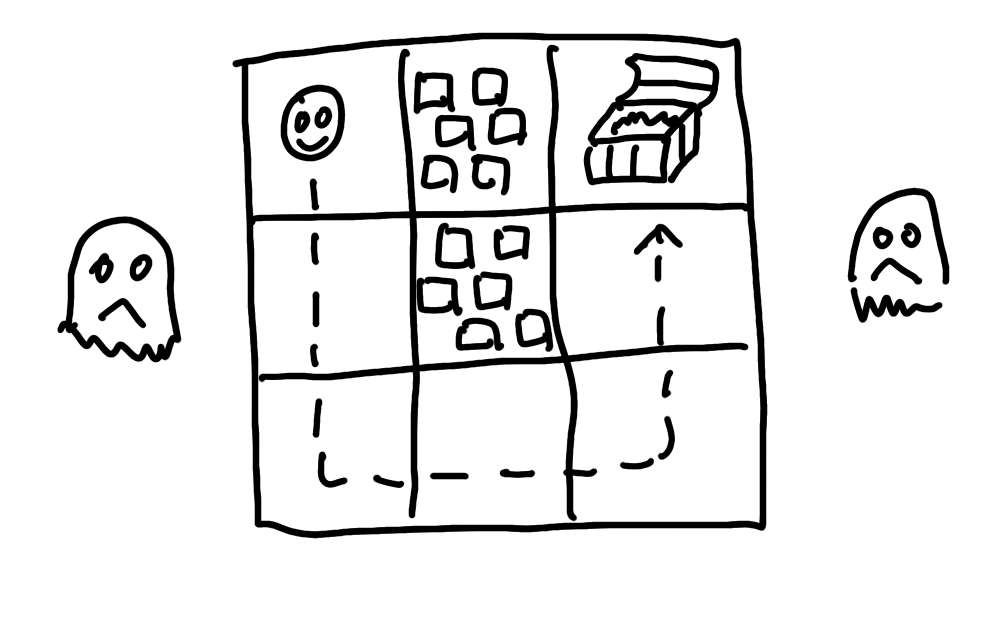
\includegraphics[width=35mm]{images/maze.png}};
\end{tikzpicture}

\end{frame}

\begin{frame}
  \centerline{Монадът Maybe}
\end{frame}


\begin{frame}[fragile]
  \frametitle{Maybe}

\begin{lstlisting}[language=Haskell]
data Maybe a = Nothing | Just a

left :: Game -> Maybe Game
left (Game (x, y) w) 
    | dead w (x-1,y) = Nothing
    | otherwise = Just $ Game (x-1, y) w

\end{lstlisting}

\end{frame}


\begin{frame}[fragile]
  \frametitle{Обобщение на операциите}

\begin{lstlisting}[language=Haskell]
move :: Game -> (Pos -> Pos) -> Maybe Game
move (Game p w) mv = if dead w (mv p) 
                     then Nothing 
                     else Just $ Game (mv p) w

left g = move g (\(x, y) -> (x-1, y))
right g = move g (\(x, y) -> (x+1, y))
up g = move g (\(x, y) -> (x, y-1))
down g = move g (\(x, y) -> (x, y+1))
\end{lstlisting}

\end{frame}


\begin{frame}[fragile]
  \frametitle{Разглеждане на случаи}

\begin{lstlisting}[language=Haskell]
case val of
  pattern1 -> ...
  pattern2 -> ...
\end{lstlisting}

\end{frame}



\begin{frame}[fragile]
  \frametitle{Композиране на операции}

\begin{lstlisting}[language=Haskell]
walk2 = case (down myWorld) of
             Nothing -> Nothing
             Just w -> case (down w) of
                        Nothing -> Nothing
                        Just w' -> case (right w') of
                                    Nothing -> Nothing
                                    Just w'' -> Just w''

\end{lstlisting}

\begin{itemize}
  \item А преди беше:
\end{itemize}

\begin{lstlisting}[language=Haskell]
walk1 = myWorld->>down->>down->>right->>right->>up->>up
\end{lstlisting}


\end{frame}


\begin{frame}[fragile]
  \frametitle{Какво ни дават монадите?}

\begin{lstlisting}[language=Haskell]
Just myWorld >>= down >>= down >>= right >>= 
     right >>= up >>= up
\end{lstlisting}

\begin{itemize}
  \item Дефиниция на \verb#>>=#
\end{itemize}

\begin{lstlisting}[language=Haskell]
ghci>:info >>=
type Monad :: (* -> *) -> Constraint
class Applicative m => Monad m where
  (>>=) :: m a -> (a -> m b) -> m b
\end{lstlisting}
\end{frame}


\begin{frame}[fragile]
  \frametitle{Как е дефиниранo това?}

\begin{lstlisting}[language=Haskell]
--(>>=) :: m a -> (a -> m b) -> m b
instance Monad Maybe where
  ...
Nothing >>= f = Nothing
Just x >>= f = f x
\end{lstlisting}


\begin{lstlisting}[language=Haskell]
Just myWorld >>= down >>= down >>= right 
             >>=right >>= up >>= up
\end{lstlisting}

\end{frame}

\begin{frame}
  \centerline{Either: Maybe с допълнителна информация}
\end{frame}

\begin{frame}[fragile]
  \frametitle{Either}

\begin{lstlisting}[language=Haskell]
data Either a b = Left a | Right b

  --(>>=) :: m a -> (a -> m b) -> m b
  --instance Monad Maybe where
  ...
Right x >>= f = f x
Left x >>= f = Left x
\end{lstlisting}

\end{frame}


\begin{frame}[fragile]
  \frametitle{Either}

\begin{lstlisting}[language=Haskell]
move :: Game -> (Pos -> Pos) -> Either String Game
move (Game p w) mv = if dead w (mv p) 
                     then Left "Player died!" 
                     else Right $ Game (mv p) w
\end{lstlisting}

\begin{itemize}
  \item По подобие на изключенията, дава възможност да се предаде информация за грешката
\end{itemize}

\end{frame}


\begin{frame}[fragile]
  \frametitle{Either}


\begin{lstlisting}[basicstyle=\tiny\ttfamily,language=Haskell]
movee :: Game -> (Pos -> Pos) -> Either String Game
movee (Game (x,y) w) mv 
  | newx < 0 || newx >= length w ||
    newy < 0 || newy >= length w    = Left "Dropped offworld."
  | (w !! newy) !! newx == Wall     = Left "Hit a wall."
  | otherwise                       = Right $ Game (newx,newy) w
  where (newx,newy) = mv (x,y)

\end{lstlisting}

\begin{lstlisting}[language=Haskell]
Right myWorld >>= down >>= down >>= right 
              >>=right >>= up >>= up
\end{lstlisting}

\end{frame}



\begin{frame}[fragile]
  \frametitle{Какво са монадите?}

  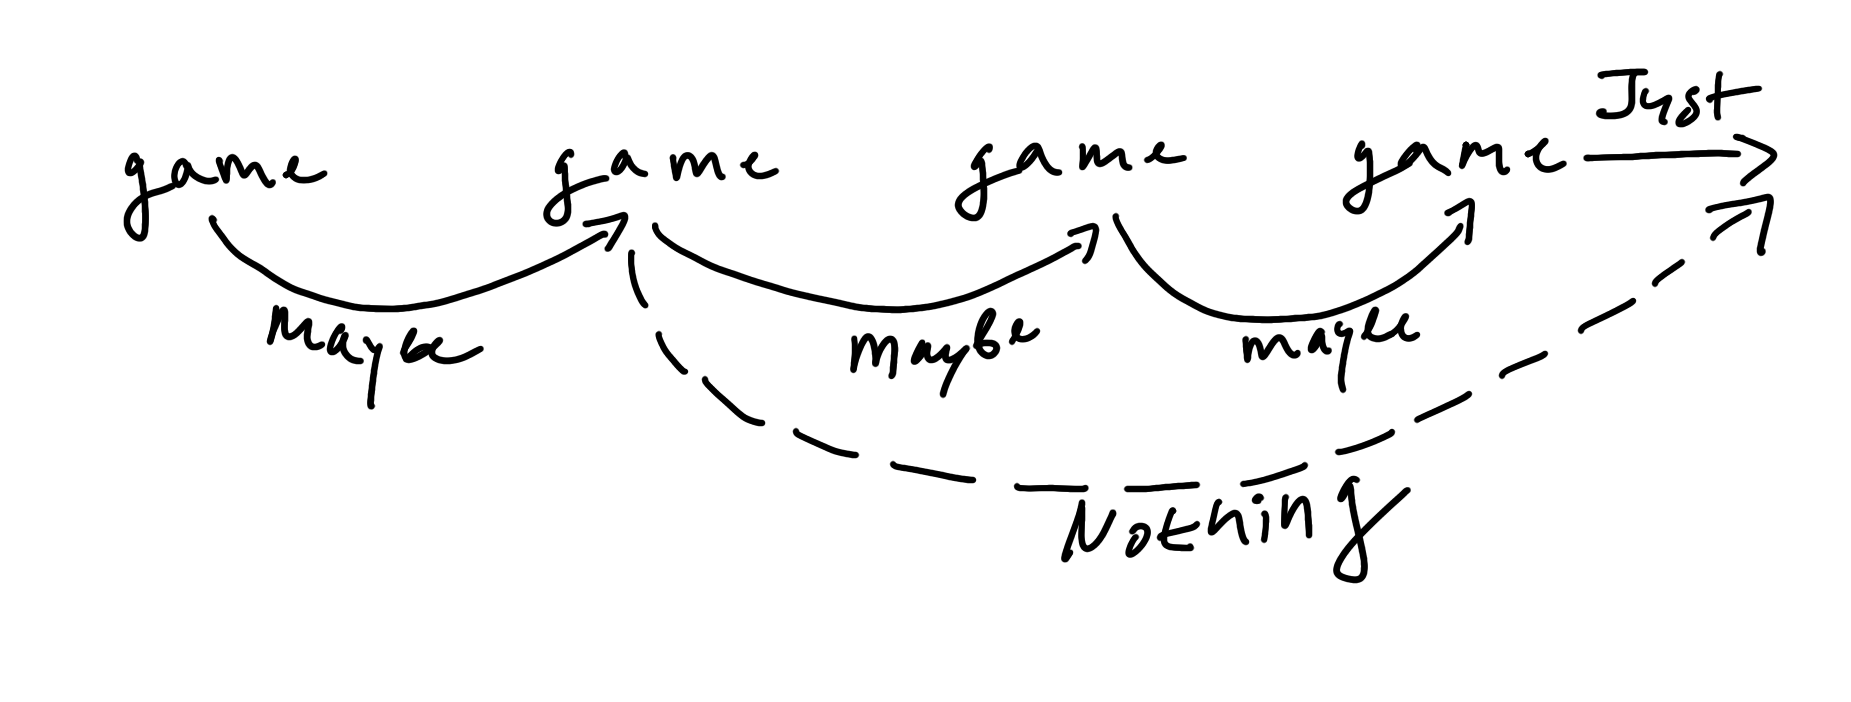
\includegraphics[width=110mm]{images/composition}

\begin{itemize}
  \item ``Закичват'' стойности с допълнителна информация (embelishment)
  \item Дефинират композиция на операции
\end{itemize}

\end{frame}

\section{Вход/Изход}
\begin{frame}
  \centerline{Вход/Изход}
\end{frame}


\begin{frame}[fragile]
  \frametitle{Какво е IO монада?}
\begin{itemize}
  \item Обвързва ``чиста'' стойност с операциите за прочитането ѝ
  \item Позволява композиране на последователност от операции, зависими от вход и изход
  \item Тъй като смисълът от някои операции е да произведат страничен ефект, понятието ``стойност'' за тях няма смисъл (\texttt{void}). Това изключва възможността на тях да гледаме ``функционално''
  \item Стойността, получена чрез входна операция, не е ``чиста'', но изчислението с нея може да е чисто
\end{itemize}

\begin{lstlisting}[language=Haskell]
io = do 
    x <- getLine
    putStrLn ("You entered: " ++  x)
    putStrLn "Thank you!"
    return x
\end{lstlisting}
  
\end{frame}


\begin{frame}[fragile]
  \frametitle{do нотация}
\begin{itemize}
  \item Опростява писането при композиране на монадични операции
  \item Подчертва последователността на операциите
  \item Улеснява извличането на чисти стойности
  \item let vs. \verb#<-#
\end{itemize}
\begin{lstlisting}[basicstyle=\small,language=Haskell]
test = do
    line1 <- getLine
    let h1 = head line1
    line2 <- getLine
    let h2 = head line1
    let ascii = max (ord h1) (ord h2)
    return ascii
\end{lstlisting}
\end{frame}

\begin{frame}[fragile]
  \frametitle{IO монада}
\begin{itemize}
  \item Така и така сме в \verb#do#, защо да не изведем нещо?
\end{itemize}
\begin{lstlisting}[basicstyle=\small,language=Haskell]
test = do
    line1 <- getLine
    let h1 = head line1
    putStrLn $ "First letter: " ++ [h1]
    line2 <- getLine
    let h2 = head line2
    putStrLn $ "Second letter: " ++ [h2]
    let ascii = max (ord h1) (ord h2)
    putStrLn $ "Max ascii: " ++ (show ascii)
    return ascii
\end{lstlisting}
\end{frame}






\begin{frame}[fragile]
    \frametitle{}
  
  \centerline{Благодаря за вниманието!}
\newcommand{\license}[1]{
  \begin{tikzpicture}[remember picture,overlay]
      \node[xshift=0mm,yshift=13mm,anchor=south east] at (current page.south east)
      {\tiny{Материалите са разработени от Калин Георгиев за курсовете по програмиране на ФМИ, СУ}};
      \node[xshift=0mm,yshift=10mm,anchor=south east] at (current page.south east)
      {\tiny{Creative Commons Attribution-NonCommercial-ShareAlike 4.0 International}};
      \node[xshift=0mm,yshift=5mm,anchor=south east] at (current page.south east){%
      \includegraphics[width=30mm]{{#1}/license}};
    \end{tikzpicture}
}
\license{../../..}
 
\end{frame}  


\end{document}


\begin{columns}[t]
  \begin{column}{0.2\textwidth}

\relscale{0.63}
\begin{lstlisting}
\end{lstlisting}
\relscale{1}

  \end{column}
  \begin{column}{0.8\textwidth}

  \end{column}
\end{columns}


